\chapter{计算机立体视觉基础}
\label{cha:chapVSLAM}
\section{引言}
\label{sec:chapVSLAM.1}
引言引言
\section{图像处理}
\section{相机模型}
相机能够将三维世界中的坐标点映射到二维图像平面中,这个过程可以利用数学建立几何模型进行描述,此类模型有很多种, SLAM中最常用的模
型为针孔模型。该模型描述了一束光通过针孔后,在针孔背面投影成像的关系,再同时考虑透镜的存在,会使得光线投影产生畸变,本文将利用针
孔和畸变两个模型来描述整个过程。

\subsection{刚体运动数学模型}
相机也可以看成三维空间中的刚体,即保证了同一个向量在各个坐标系下的长度和夹角都不会发生变化,因此需要考虑相机的位姿,即旋转和平移。
对于平移可以利用向量来表示,旋转则利用旋转矩阵,旋转向量,欧拉角,四元数等方式来描述,本文也将主要说明旋转过程的数学描述。

\textbf{旋转矩阵:}对于任意向量{~p~},在两个坐标系的描述为:
\begin{equation}
  \left[\mathbf{e}_{1}, \mathbf{e}_{2}, \mathbf{e}_{3}\right]\left[\begin{array}{l}{a_{1}} \\ {a_{2}} \\ {a_{3}}\end{array}\right]=\left[\mathbf{e}_{1}^{\prime}, \mathbf{e}_{2}^{\prime}, \mathbf{e}_{3}^{\prime}\right]\left[\begin{array}{c}{a_{1}^{\prime}} \\ {a_{2}^{\prime}} \\ {a_{3}^{\prime}}\end{array}\right]
\end{equation}

等式两边同时左乘$\left[\begin{array}{ccc}{\mathbf{e}_{1}^{T},} & {\mathbf{e}_{2}^{T},} & {\mathbf{e}_{3}^{T}}\end{array}\right]^{T}$可得
\begin{equation}
\left[\begin{array}{l}{a_{1}} \\ {a_{2}} \\ {a_{3}}\end{array}\right]=\left[\begin{array}{lll}{e_{1}^{T} e_{1}^{\prime}} & {e_{1}^{T} e_{2}^{\prime}} & {e_{1}^{T} e_{3}^{\prime}} \\ {e_{2}^{T} e_{1}^{\prime}} & {e_{2}^{T} e_{2}^{\prime}} & {e_{2}^{T} e_{3}^{\prime}} \\ {e_{3}^{T} e_{1}^{\prime}} & {e_{3}^{T} e_{2}^{\prime}} & {e_{3}^{T} e_{3}^{\prime}}\end{array}\right]\left[\begin{array}{c}{a_{1}^{\prime}} \\ {a_{2}^{\prime}} \\ {a_{3} ;}\end{array}\right]=\mathbf{R a}^{\prime}
\end{equation}

对于旋转矩阵R,即可描述旋转过程,并且R可以定义为特殊正交群:
\begin{equation}
  S O(n)=\left\{\mathbf{R} \in R^{n \times n} | \mathbf{R} \mathbf{R}^{T}=\mathbf{I}, \operatorname{det}(\mathbf{R})=1\right\}
\end{equation}

\textbf{旋转向量:}旋转矩阵在描述旋转时存在参数冗余和自身约束的问题,因此提出一个更加紧凑的数学描述$\theta_{n}$,旋转向量方向为旋转轴{~n~},
大小为旋转角$\theta$。旋转向量和旋转矩阵的转换可以用罗德里格斯公式表示:
\begin{equation}
  \mathbf{R}=\cos \theta \mathbf{I}+(1-\cos \theta) \mathbf{n} \mathbf{n}^{T}+\sin \theta \mathbf{n}^{\wedge}
\end{equation}

反之则有
\begin{equation}
  \operatorname{tr}(\mathbf{R})=\cos \theta \operatorname{tr}(\mathbf{I})+(1-\cos \theta) \operatorname{tr}\left(\mathbf{n} \mathbf{n}^{T}\right)+\sin \theta \operatorname{tr}\left(\mathbf{n}^{\wedge}\right)=1+2 \cos \theta
\end{equation}

\textbf{欧拉角:}将旋转运动分解成分别绕三个坐标轴的旋转($[r, p, y]^{T}$)来表示的,三个旋转的总和即为总的旋转,表述最为直观。

\textbf{四元数:}由于欧拉角和旋转向量存在奇异性,且不存在不带奇异性的三维向量描述方式,因此提出四元数这种紧凑且没有奇异性的数学
描述。四元数可以描述为:
\begin{equation}
  \mathbf{q}=q_{0}+q_{1} i+q_{2} j+q_{3} k=\{s, \mathbf{v}\}
\end{equation}
可以用单位四元数来描述空间中的任意旋转,假设旋转的描述为$\theta_{n}$,则:
\begin{equation}
  \mathbf{q}=\left[\cos \frac{\theta}{2}, n_{x} \sin \frac{\theta}{2}, n_{y} \sin \frac{\theta}{2}, n_{z} \sin \frac{\theta}{2}\right]^{T}
\end{equation}
旋转描述为R时,则:
\begin{equation}
\mathbf{R}=\left[\begin{array}{ccc}{1-2 q_{2}^{2}-2 q_{3}^{2}} & {2 q_{1} q_{2}-2 q_{0} q_{3}} & {2 q_{1} q_{3}+2 q_{0} q_{2}} \\ {2 q_{1} q_{2}+2 q_{0} q_{3}} & {1-2 q_{1}^{2}-2 q_{3}^{2}} & {2 q_{2} q_{3}-2 q_{0} q_{1}} \\ {2 q_{1} q_{3}-2 q_{0} q_{2}} & {2 q_{2} q_{3}+2 q_{0} q_{1}} & {1-2 q_{1}^{2}-2 q_{2}^{2}}\end{array}\right]
\end{equation}
反之则有:
\begin{equation}
  q_{0}=\frac{\sqrt{\operatorname{tr}(\mathbf{R})+1}}{2}, q_{1}=\frac{m_{23}-m_{32}}{4 q_{0}}, q_{2}=\frac{m_{31}-m_{13}}{4 q_{0}}, q 3=\frac{m_{12}-m_{21}}{4 q_{0}}
\end{equation}
通过以上方式都可以描述刚性运动中的旋转过程R,结合物体的平移t,则变化后的坐标为:
\begin{equation}
  \mathbf{a}^{\prime}=\mathbf{R} \mathbf{a}+\mathbf{t}
\end{equation}

在实际的使用中,由于以上等式非线性,可以引入齐次坐标T,可以将上式改成:
\begin{equation}
\left[\begin{array}{l}{\mathbf{a}^{\prime}} \\ {1}\end{array}\right]=\left[\begin{array}{ll}{\mathbf{R}} & {\mathbf{t}} \\ {\mathbf{0}^{T}} & {1}\end{array}\right]\left[\begin{array}{l}{\mathbf{a}^{\prime}} \\ {1}\end{array}\right]=\mathbf{T}\left[\begin{array}{l}{\mathbf{a}} \\ {1}\end{array}\right]
\end{equation}

对于变换矩阵T,可以定义为特殊欧氏群:
\begin{equation}
S E(3)=\left\{T=\left[\begin{array}{cc}{\mathbf{R}} & {\mathbf{t}} \\ {\mathbf{0}^{T}} & {1}\end{array}\right] \in R^{4 \times 4} | \mathbf{R} \in S O(3), t \in R^{3}\right\}
\end{equation}




\subsection{针孔相机模型}
对于针孔相机模型,如图~\ref{fig:2VSLAM_pinehole}所示,(其中f为相机焦距)存在4个坐标系分别为:世界坐标系,相机坐标系,图像坐
标系和像素坐标系,对于真实世界中的空间点$P_w$($X_w$,$Y_w$,$Z_w$),其对应的相机坐标系坐标为$P_c$($C_w$,$C_w$,$C_w$),
对应的图像坐标系为$P^{'}$($X^{'}$,$Y^{'}$),对应的像素坐标系为p(u,v)。
\begin{figure}[H] % use float package if you want it here
  \centering
  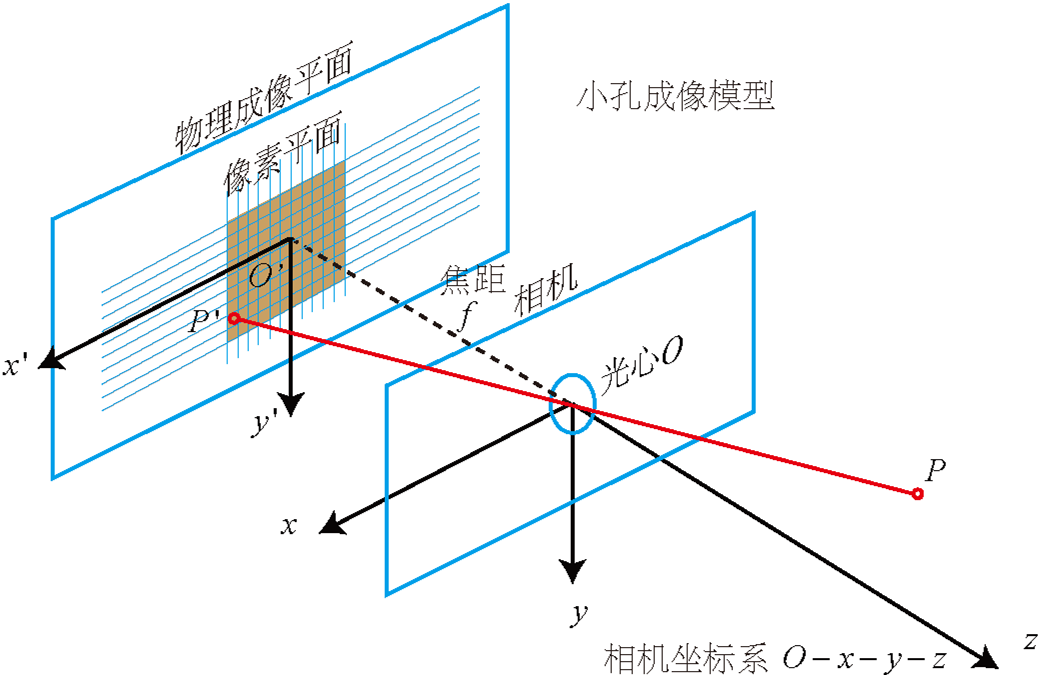
\includegraphics[height=6cm]{2VSLAM_pinehole.png}
  \caption{针孔相机模型}
  \label{fig:2VSLAM_pinehole}
\end{figure}
对于世界坐标系到相机坐标系之间的转化:
\begin{equation}
  \left[\begin{array}{l}{X c} \\ {Y_{C}} \\ {Z_{C}}\end{array}\right]=R\left[\begin{array}{l}{X w} \\ {Y w} \\ {Z w}\end{array}\right]+t
  \label{equ:world2cam}
\end{equation}
对于相机坐标系到图像坐标系之间的转化,可以利用如图~\ref{fig:2VSLAM_similartri}所示的相似三角形来求解:
\begin{equation}
  \begin{split}
    \frac{Z c}{f}=\frac{X c}{X^{'}}=\frac{Y c}{Y^{'}}\\
    \left\{\begin{array}{l}{X^{\prime}=f \frac{X c}{Z c}} \\ {Y^{\prime}=f \frac{Y c}{Z c}}\end{array}\right.
\end{split}
\label{equ:cam2photo}
\end{equation}
对于图像坐标系到像素坐标系的转化,如图~\ref{fig:2VSLAM_pixeltrans}所示:
\begin{equation}
  \begin{split}
    \left\{\begin{array}{l}{u=\frac{X^{\prime}}{d_{x}}+u_{o}} \\ {v=\frac{Y^{\prime}}{d_{y}}+v_{o}}\end{array}\right.\\
    \left[\begin{array}{l}{u} \\ {v} \\ {1}\end{array}\right]=\left[\begin{array}{ccc}{\frac{1}{d_{x}}} & {0} & {u_{o}} \\ {0} & {\frac{1}{d_{x}}} & {v_{o}} \\ {0} & {0} & {1}\end{array}\right]\left[\begin{array}{c}{X^{\prime}} \\ {Y^{\prime}} \\ {1}\end{array}\right]
  \end{split}
  \label{equ:photo2pixel}
\end{equation}
\begin{figure}[H]
  \centering%
  \subcaptionbox{相机坐标系到图像坐标系转换\label{fig:2VSLAM_similartri}}{%    
    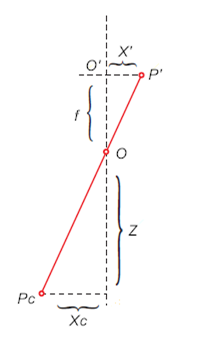
\includegraphics[height=4cm]{2VSLAM_similartri.png}}\hspace{6em}%
  \subcaptionbox{图像坐标系到像素坐标系转换\label{fig:2VSLAM_pixeltrans}}{%    
    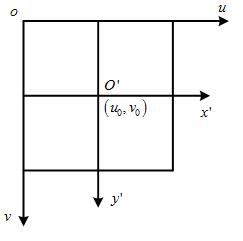
\includegraphics[height=4cm]{2VSLAM_pixeltrans.png}}
  \caption{坐标系转化示意图}
  \label{fig:trans}
\end{figure}
其中$d_x$,$d_y$分别表示沿着x,y轴的实际物理尺寸,($u_o$,$v_o$)表示光心对应到像素坐标系得到坐标.由公式~\ref{equ:cam2photo}和
~\ref{equ:photo2pixel}可以转化得到相机坐标系到像素坐标系的关系:
\begin{equation}
Z c\left[\begin{array}{l}{u} \\ {v} \\ {1}\end{array}\right]=\left[\begin{array}{ccc}{\frac{f}{d_{x}}} & {0} & {u_{0}} \\ {0} & {\frac{f}{d_{y}}} & {v_{0}} \\ {0} & {0} & {1}\end{array}\right]\left[\begin{array}{c}{X_{c}} \\ {Y_{c}} \\ {Z_{c}}\end{array}\right]=\left[\begin{array}{ccc}{f_{x}} & {0} & {u_{0}} \\ {0} & {f_{y}} & {v_{0}} \\ {0} & {0} & {1}\end{array}\right]\left[\begin{array}{c}{X_{c}} \\ {Y_{c}} \\ {Z_{c}}\end{array}\right]=K\left[\begin{array}{c}{X_{c}} \\ {Y_{c}} \\ {Z_{c}}\end{array}\right]
  \label{equ:cam2pixel}
\end{equation}
由公式~\ref{equ:world2cam}和~\ref{equ:cam2pixel}得到世界坐标系到像素坐标系的转化关系为:
\begin{equation}
Z c\left[\begin{array}{l}{u} \\ {v} \\ {1}\end{array}\right]=K(R P w+t)=K\left(R\left[\begin{array}{l}{X w} \\ {Y w} \\ {Z w}\end{array}\right]+t\right)
\end{equation}
其中K表示相机内参矩阵,R,t表示相机外参。


\subsection{相机畸变模型}
为了使得相机产生更好的成像效果,会加入透镜,透镜的加入对成像过程中光线的传播产生影响会引入径向畸变,这类畸变可以用于距中心的距离
有关的二次及高次多项式函数进行修正。
\begin{equation}
\left\{\begin{array}{l}{x_{r a d}=x\left(1+k_{1} r^{2}+k_{2} r^{4}+k_{3} r^{6}\right)} \\ {y_{r a d}=y\left(1+k_{1} r^{2}+k_{2} r^{4}+k_{3} r^{6}\right)}\end{array}\right.
\end{equation}

在相机的组装过程中,由于不可能保证透镜和相机得到成像平面得到的完全平行,也会引入切向畸变,可以使用两个参数$p_1$,$p_2$来进行修
正。
\begin{equation}
  \left\{\begin{array}{l}{x_{\tan }=x+2 p_{1} x y+p_{2}\left(r^{2}+2 x^{2}\right)} \\ {y_{\tan }=y+p_{1}\left(r^{2}+2 y^{2}\right)+2 p_{2} \pi y}\end{array}\right.
\end{equation}

联合公式,对于相机坐标系中的点P(X,Y,Z),通过以上5个畸变参数找到该点在像素坐标系上的正确位置。
\begin{equation}
  \left\{\begin{array}{l}{x_{\text {corrected}}=x\left(1+k_{1} r^{2}+k_{2} r^{4}+k_{3} r^{6}\right)+2 p_{1} \pi y+p_{2}\left(r^{2}+2 x^{2}\right)} \\ {y_{\text {corrected}}=y\left(1+k_{1} r^{2}+k_{2} r^{4}+k_{3} r^{6}\right)+p_{1}\left(r^{2}+2 y^{2}\right)+2 p_{2} x y}\end{array}\right.
\end{equation}


